\documentclass[a4paper,10pt]{article}

\usepackage[brazilian]{babel}
\usepackage[left=2.5cm,right=2.5cm,top=3cm,bottom=2.5cm]{geometry}
\usepackage{mathtools}
\usepackage{amsthm}
\usepackage{amsmath}
%\usepackage{nccmath}
\usepackage{amssymb}
\usepackage{amsfonts}
\usepackage{physics}
%\usepackage{dsfont}
%\usepackage{mathrsfs}

\usepackage{titling}
\usepackage{indentfirst}

\usepackage{bm}
\usepackage[dvipsnames]{xcolor}
\usepackage{cancel}

\usepackage{xurl}
\usepackage[colorlinks=true]{hyperref}

\usepackage{float}
\usepackage{graphicx}
%\usepackage{tikz}
\usepackage{caption}
\usepackage{subcaption}

%%%%%%%%%%%%%%%%%%%%%%%%%%%%%%%%%%%%%%%%%%%%%%%%%%%

\newcommand{\eps}{\epsilon}
\newcommand{\vphi}{\varphi}
\newcommand{\cte}{\text{cte}}

\newcommand{\N}{\mathbb{N}}
\newcommand{\Z}{\mathbb{Z}}
\newcommand{\Q}{\mathbb{Q}}
\newcommand{\R}{\vb{R}}
\newcommand{\C}{\mathbb{C}}
\renewcommand{\S}{\hat{S}}
%\renewcommand{\H}{\s{H}}

\renewcommand{\a}{\vb{a}}
\newcommand{\nn}{\hat{n}}
\renewcommand{\d}{\dagger}
\newcommand{\up}{\uparrow}
\newcommand{\down}{\downarrow}

\newcommand{\0}{\vb{0}}
%\newcommand{\1}{\mathds{1}}
\newcommand{\E}{\vb{E}}
\newcommand{\B}{\vb{B}}
\renewcommand{\v}{\vb{v}}
\renewcommand{\r}{\vb{r}}
\renewcommand{\k}{\vb{k}}
\newcommand{\p}{\vb{p}}
\newcommand{\q}{\vb{q}}
\newcommand{\F}{\vb{F}}

\newcommand{\s}{\sigma}
%\newcommand{\prodint}[2]{\left\langle #1 , #2 \right\rangle}
\newcommand{\cc}[1]{\overline{#1}}
\newcommand{\Eval}[3]{\eval{\left( #1 \right)}_{#2}^{#3}}

\newcommand{\unit}[1]{\; \mathrm{#1}}

\newcommand{\n}{\medskip}
\newcommand{\e}{\quad \mathrm{e} \quad}
\newcommand{\ou}{\quad \mathrm{ou} \quad}
\newcommand{\virg}{\, , \;}
\newcommand{\ptodo}{\forall \,}
\renewcommand{\implies}{\; \Rightarrow \;}
%\newcommand{\eqname}[1]{\tag*{#1}} % Tag equation with name

\setlength{\droptitle}{-7em}

\theoremstyle{plain}
\newtheorem{theorem}{Teorema}[section]
%\newtheorem{defi}[theorem]{Definição}
\newtheorem{lemma}[theorem]{Lema}
%\newtheorem{corol}[theorem]{Corolário}
%\newtheorem{prop}[theorem]{Proposição}
%\newtheorem{example}{Exemplo}
%
%\newtheorem{inneraxiom}{Axioma}
%\newenvironment{axioma}[1]
%  {\renewcommand\theinneraxiom{#1}\inneraxiom}
%  {\endinneraxiom}
%
%\newtheorem{innerpostulado}{Postulado}
%\newenvironment{postulado}[1]
%  {\renewcommand\theinnerpostulado{#1}\innerpostulado}
%  {\endinnerpostulado}
%
%\newtheorem{innerexercise}{Exercício}
%\newenvironment{exercise}[1]
%  {\renewcommand\theinnerexercise{#1}\innerexercise}
%  {\endinnerexercise}
%
%\newtheorem{innerthm}{Teorema}
%\newenvironment{teorema}[1]
%  {\renewcommand\theinnerthm{#1}\innerthm}
%  {\endinnerthm}
%
\newtheorem{innerlema}{Lema}
\newenvironment{lema}[1]
  {\renewcommand\theinnerlema{#1}\innerlema}
  {\endinnerlema}
%
%\theoremstyle{remark}
%\newtheorem*{hint}{Dica}
%\newtheorem*{notation}{Notação}
%\newtheorem*{obs}{Observação}


\newcommand{\vac}{\ket{vac}}
\newcommand{\hh}{\tilde{h}}
\newcommand{\hhh}{\bm{\tilde{h}}}
\newcommand{\vecs}{(\s^x, \s^y, \s^z)}
\renewcommand{\ss}{\bm{\sigma}}


\title{\Huge{\textbf{Prova final - Mecânica Estatística}}}
\author{Mateus Marques}

\begin{document}

\maketitle

\section*{1) Modelo de Ising em um campo transverso}

(a) Primeiramente, observe que:
\begin{itemize}
\item Pelas relações de comutação de férmions, temos $[n_k, n_\ell] = 0$ para quaisquer sítios $k, \ell$.

\n

\item Em particular, a exponencial da soma $e^{\pm i\pi \sum_{k<j} n_k}$ pode ser separada no produto $\prod_{k<j} e^{\pm i\pi n_k}$, pois todos os operadores $n_k$ comutam entre si.

\n

\item Como $n_k^2 = n_k$ pelo princípio de Pauli, temos também $n_k^p = n_k$ para qualquer natural $p\geq 1$. Assim:
$$
e^{\pm i\pi n_k} = 1 + \sum_{p=1}^{\infty} \frac{(\pm i\pi n_k)^p}{p!} = 1+ \qty( \sum_{p=1}^{\infty} \frac{(\pm i\pi)^p}{p!} ) n_k = 1 + (e^{\pm i \pi} - 1) n_k = 1 - 2 n_k = - \s_j^z,
$$
$$
e^{\pm i\pi \sum_{k<j} n_k} = \prod_{k<j} e^{\pm i\pi n_k} = \prod_{k<j} (-\s_k^z).
$$

\end{itemize}

Temos então que
$$
\sigma_j^x = \frac{\qty(\sigma_j^+ + \sigma_j^-)}{2} =
e^{i\pi \sum_{k<j} n_k} f_j^\d + e^{-i\pi \sum_{k<j} n_k} f_j =
\qty[\prod_{k<j} (-\s_k^z)] \qty(f_j^\d + f_j).
$$

\n

Substituindo $\s_j^x$ acima e $\s_j^z = 2 n_j - 1$ na hamiltoniana:
$$
H = -J \sum_{j} \s_j^x \s_{j+1}^x + h \sum_{j} \s_j^z =
-J \sum_{j} \qty[\prod_{k<j} \big(\s_k^z\big)^2] (f_j+f_j^\d)(1-2n_j)(f_{j+1} + f_{j+1}^\d) + h \sum_{j} (2n_j - 1).
$$

Veja que $\big(\s_k^z\big)^2 = 1$ e que
$$
(f_j+f_j^\d)(1-2n_j) = (f_j+f_j^\d)(1-2 f_j^\d f_j) =
f_j+f_j^\d - 2 f_j f_j^\d f_j =
f_j+f_j^\d - 2 (1 - f_j^\d f_j) f_j =
f_j^\d - f_j.
$$

\n

Assim, temos
$$
H =
-J \sum_{j} \qty[ (f_j^\d - f_j) (f_{j+1} + f_{j+1}^\d) - g (2 f_j^\d f_j - 1)] \implies
$$

\begin{equation} \label{eq:hamil_transvising}
\boxed{ H =
-J \sum_{i} \qty[ f_i^\d f_{i+1}^\d + f_{i+1} f_i + f_i^\d f_{i+1} + f_{i+1}^\d f_i - 2 g f_i^\d f_i + g]. }
\end{equation}

\n\n

(b) Tomando agora as transformadas $f_j^\d = \frac{1}{\sqrt{N}} \sum_{k} e^{-ikja} f_k^\d$, $f_j = \frac{1}{\sqrt{N}} \sum_{k'} e^{ik'ja} f_{k'}$ e lembrando da relação $\sum_{j} e^{-i(k-k')ja} = N \delta_{k,k'}$ para a transformada discreta de Fourier da função $\delta$, temos
$$
H =
-J \sum_{i} \qty[ \Big( f_{i+1} f_i + f_{i+1}^\d f_i + \hc \Big) - 2 g f_i^\d f_i + g] =
$$
$$
H =
-\frac{J}{N} \sum_{j} \sum_{k,k'} \qty{ \qty[ e^{ik'a} e^{i(k+k')ja} f_{k'} f_k + e^{ik'a} e^{-i(k-k')ja} f_k^\d f_{k'} + \hc ] - 2g \, e^{-i(k-k')ja} f_k^\d f_{k'} + g \, \delta_{k,k'}} =
$$
$$
=
-J \sum_{k,k'} \qty{ \qty[ e^{ik'a} \delta_{-k,k'} f_{k'} f_k + e^{ik'a} \delta_{k,k'} f_k^\d f_{k'} + \hc ] - 2g \, \delta_{k,k'} f_k^\d f_{k'} + g \, \delta_{k,k'}} =
$$
$$
=
-J \sum_{k} \qty{ \qty[ e^{-ika} f_{-k} f_k + e^{ika} f_k^\d f_{k} + \hc ]
- 2 g f_k^\d f_k + g } =
$$
$$
=
-J \sum_{k} \qty{ \qty[ e^{-ika} f_{-k} f_k + \boxed{e^{ika} f_k^\d f_{k}} + e^{ika} f_{k}^\d f_{-k}^\d + \boxed{e^{-ika} f_k^\d f_{k}} ]
\boxed{- 2 g f_k^\d f_k} + g } =
$$
$$
=
J \sum_{k} \qty{ 2 \qty[g - \cos(ka)] f_k^\d f_{k} - \qty( e^{-ika} f_{-k} f_k + e^{ika} f_{k}^\d f_{-k}^\d ) - g }.
$$

O termo acima em parênteses que possui exponenciais complexas pode ser reescrito como (fazendo a média com outra somatória em $-k$)
$$
\sum_{k} \qty( e^{-ika} f_{-k} f_k + e^{ika} f_{k}^\d f_{-k}^\d ) =
\frac{1}{2} \sum_{k} \qty( e^{-ika} f_{-k} f_k + e^{ika} f_{k}^\d f_{-k}^\d ) \; + \;
\frac{1}{2} \sum_{k} \qty( e^{ika} f_{k} f_{-k} + e^{-ika} f_{-k}^\d f_{k}^\d ) =
$$
$$
=
\frac{1}{2} \sum_{k} \qty( e^{-ika} f_{-k} f_k - e^{ika} f_{-k}^\d f_{k}^\d ) \; + \;
\frac{1}{2} \sum_{k} \qty( -e^{ika} f_{-k} f_k + e^{-ika} f_{-k}^\d f_{k}^\d ) =
$$
$$
= \sum_{k} \qty{
\qty(\frac{e^{-ika} - e^{ika} }{2}) f_{-k} f_k + \qty(\frac{e^{-ika} - e^{ika} }{2}) f_{-k}^\d f_k^\d }
= \sum_{k} \qty[ -i \sin(ka) \qty(
f_{-k}^\d f_k^\d + f_{-k} f_k ) ].
$$

\n

Portanto, a hamiltoniana fica
$$
\boxed{ H =
J \sum_{k} \qty{ 2 \qty[g - \cos(ka)] f_k^\d f_{k} + i \, \sin(ka) \qty( f_{-k}^\d f_k^\d + f_{-k} f_{k} ) - g }. }
$$

\n\n

(c) Desenvolvendo a multiplicação de matriz pedida, temos
$$
\begin{pmatrix}
f_k^\d & f_{-k}
\end{pmatrix}
\begin{pmatrix}
g-\cos(ka) & -i\sin(ka) \\
i\sin(ka) & -[g-\cos(ka)]
\end{pmatrix}
\begin{pmatrix}
f_k \\ f_{-k}^\d
\end{pmatrix}
=
\begin{pmatrix}
f_k^\d & f_{-k}
\end{pmatrix}
\begin{pmatrix}
[g-\cos(ka)] f_k - i \sin(ka) f_{-k}^\d \\ -[g-\cos(ka)] f_{-k}^\d + i \sin(ka) f_k
\end{pmatrix}
=
$$
$$
=
[g-\cos(ka)] f_k^\d f_k - i\sin(ka) \underbrace{f_k^\d f_{-k}}_{=-f_{-k}^\d f_k^\d}
- [g-\cos(ka)] \underbrace{f_{-k} f_{-k}^\d}_{=1-f_{-k}^\d f_{-k}} + i \sin(ka) f_{-k} f_k =
$$
$$
=
[g-\cos(ka)] (f_k^\d f_k + \boxed{f_{-k}^\d f_{-k}}) - g + \boxed{\cos(ka)} + i\sin(ka) (f_{-k}^\d f_{-k}^\d + f_{-k} f_k).
$$

Considerando os dois termos acima destacados em uma caixa, quando se realiza a somatória em $k$ eles se simplificam:
$$
\sum_{k} f_{-k}^\d f_{-k} = \sum_{k} f_{k}^\d f_k, \quad (\text{trocando a somatória por} \, -k),
$$
$$
\sum_{k} \cos(ka) = \frac{1}{2} \sum_{k} e^{ika} + \frac{1}{2} \sum_{k} e^{-ika} = 0,
$$
pois $\sum_{k} e^{\pm ika(j-j')} = N \delta_{j,j'} = N \delta_{(j-j', 0)} \implies \sum_{k} e^{\pm ika} = \delta_{1,0} = 0$.

\n

Dessa maneira, esses cálculos mostram que a hamiltoniana se reescreve como
$$
J \sum_{k}
\begin{pmatrix}
f_k^\d & f_{-k}
\end{pmatrix}
\begin{pmatrix}
g-\cos(ka) & -i\sin(ka) \\
i\sin(ka) & -g+\cos(ka)
\end{pmatrix}
\begin{pmatrix}
f_k \\ f_{-k}^\d
\end{pmatrix}
=
$$
$$
= J \sum_{k} \qty{ 2[g-\cos(ka)] f_k^\d f_k + i\sin(ka) \Big(f_{-k}^\d f_{-k}^\d + f_{-k} f_k\Big) - g } =
H.
$$

\n

Usando a transformação de Bogoliubov explicitada
$$
f_k = \cos(\frac{\theta_k}{2}) \gamma_k + i \sin(\frac{\theta_k}{2}) \gamma_{-k}^\d \implies
\begin{pmatrix}
f_k \\ f_{-k}^\d
\end{pmatrix}
=
\begin{pmatrix}
\cos(\frac{\theta_k}{2}) & i \sin(\frac{\theta_k}{2}) \\
i \sin(\frac{\theta_k}{2}) & \cos(\frac{\theta_k}{2})
\end{pmatrix}
\begin{pmatrix}
\gamma_k \\ \gamma_{-k}^\d
\end{pmatrix} ,
$$
com $\theta_{-k} = -\theta_k$, temos
$$
\begin{pmatrix}
f_k^\d & f_{-k}
\end{pmatrix}
\begin{pmatrix}
g-\cos(ka) & -i\sin(ka) \\
i\sin(ka) & -[g-\cos(ka)]
\end{pmatrix}
\begin{pmatrix}
f_k \\ f_{-k}^\d
\end{pmatrix}
=
$$
$$
=
\begin{pmatrix}
\gamma_k^\d & \gamma_{-k}
\end{pmatrix}
\begin{pmatrix}
\cos(\frac{\theta_k}{2}) & -i \sin(\frac{\theta_k}{2}) \\
-i \sin(\frac{\theta_k}{2}) & \cos(\frac{\theta_k}{2})
\end{pmatrix}
\begin{pmatrix}
g-\cos(ka) & -i\sin(ka) \\
i\sin(ka) & -[g-\cos(ka)]
\end{pmatrix}
\begin{pmatrix}
\cos(\frac{\theta_k}{2}) & i \sin(\frac{\theta_k}{2}) \\
i \sin(\frac{\theta_k}{2}) & \cos(\frac{\theta_k}{2})
\end{pmatrix}
\begin{pmatrix}
\gamma_k \\ \gamma_{-k}^\d
\end{pmatrix}.
$$

Portanto, basta que efetuemos as multiplicações de matrizes:
$$
\begin{pmatrix}
g-\cos(ka) & -i\sin(ka) \\
i\sin(ka) & -[g-\cos(ka)]
\end{pmatrix}
\begin{pmatrix}
\cos(\frac{\theta_k}{2}) & i \sin(\frac{\theta_k}{2}) \\
i \sin(\frac{\theta_k}{2}) & \cos(\frac{\theta_k}{2})
\end{pmatrix}
=
$$
$$
\begin{pmatrix}
[g-\cos(ka)] \cos(\frac{\theta_k}{2}) + \sin(ka) \sin(\frac{\theta_k}{2}) &
[g-\cos(ka)] i \sin(\frac{\theta_k}{2}) - i \sin(ka) \cos(\frac{\theta_k}{2}) \\
-[g-\cos(ka)] i \sin(\frac{\theta_k}{2}) + i \sin(ka) \cos(\frac{\theta_k}{2}) &
-[g-\cos(ka)] \cos(\frac{\theta_k}{2}) - \sin(ka) \sin(\frac{\theta_k}{2})
\end{pmatrix}.
$$
$$
\begin{pmatrix}
\cos(\frac{\theta_k}{2}) & -i \sin(\frac{\theta_k}{2}) \\
-i \sin(\frac{\theta_k}{2}) & \cos(\frac{\theta_k}{2})
\end{pmatrix}
\times
$$
$$
\times
\begin{pmatrix}
[g-\cos(ka)] \cos(\frac{\theta_k}{2}) + \sin(ka) \sin(\frac{\theta_k}{2}) &
[g-\cos(ka)] i \sin(\frac{\theta_k}{2}) - i \sin(ka) \cos(\frac{\theta_k}{2}) \\
-[g-\cos(ka)] i \sin(\frac{\theta_k}{2}) + i \sin(ka) \cos(\frac{\theta_k}{2}) &
-[g-\cos(ka)] \cos(\frac{\theta_k}{2}) - \sin(ka) \sin(\frac{\theta_k}{2})
\end{pmatrix} =
$$
$$
\tiny{
\begin{pmatrix}
[g-\cos(ka)] [\cos[2](\frac{\theta_k}{2}) - \sin[2](\frac{\theta_k}{2})] +
2 \sin(ka) \sin(\frac{\theta_k}{2}) \cos(\frac{\theta_k}{2}) &
i [g-\cos(ka)] 2 \sin(\frac{\theta_k}{2}) \cos(\frac{\theta_k}{2}) - i \sin(ka) [\cos[2](\frac{\theta_k}{2}) - \sin[2](\frac{\theta_k}{2})] \\
- i [g-\cos(ka)] 2 \sin(\frac{\theta_k}{2}) \cos(\frac{\theta_k}{2}) + i \sin(ka) [\cos[2](\frac{\theta_k}{2}) - \sin[2](\frac{\theta_k}{2})] &
- [g-\cos(ka)] [\cos[2](\frac{\theta_k}{2}) - \sin[2](\frac{\theta_k}{2})] -
2 \sin(ka) \sin(\frac{\theta_k}{2}) \cos(\frac{\theta_k}{2})
\end{pmatrix} }
$$
$$
=
\begin{pmatrix}
\qty{[g-\cos(ka)] \cos\theta_k + \sin(ka) \sin\theta_k } &
 i \qty{[g-\cos(ka)] \sin\theta_k - \sin(ka) \cos\theta_k} \\
-i \qty{[g-\cos(ka)] \sin\theta_k - \sin(ka) \cos\theta_k} &
-\qty{[g-\cos(ka)] \cos\theta_k + \sin(ka) \sin\theta_k}
\end{pmatrix}.
$$

Olhando para a matriz acima, vemos que ela se torna diagonal quando
$$
[g-\cos(ka)] \sin\theta_k - \sin(ka) \cos\theta_k = 0 \implies
\boxed{\tan\theta_k = \frac{\sin(ka)}{g-\cos(ka)}.}
$$

Usando as relações $\cos\theta_k = \frac{1}{\sqrt{1+\tan^2\theta_k}}$ e
$\sin\theta_k = \frac{\tan\theta_k}{\sqrt{1+\tan^2\theta_k}}$, é direto mostrar que o termo da diagonal se escreve como
$$
[g-\cos(ka)] \cos\theta_k + \sin(ka) \sin\theta_k =
\sqrt{[g-\cos(ka)]^2 + \sin[2](ka)} = \lambda_k.
$$

Isso mostra então que
$$
H = J \sum_{k}
\begin{pmatrix}
\gamma_k^\d & \gamma_{-k}
\end{pmatrix}
\begin{pmatrix}
\lambda_k & 0 \\
0 & -\lambda_k
\end{pmatrix}
\begin{pmatrix}
\gamma_k \\ \gamma_{-k}^\d
\end{pmatrix} =
J \sum_{k} (\lambda_k \gamma_k^\d \gamma_k -
\lambda_k \underbrace{\gamma_{-k} \gamma_{-k}^\d}_{= 1 - \gamma_{-k}^\d \gamma_{-k}}) =
\sum_{k} \underbrace{2 J \lambda_k}_{=E_k} \qty(\gamma_k^\d \gamma_k - \frac{1}{2}).
$$

Assim, identificamos que o autovalor positivo de $M(k)$ é
$$
\boxed{ E_k = 2J \lambda_k = 2J \sqrt{1+g^2-2g\cos(ka)}. }
$$

\n

Na Figura \ref{fig:transv_ising2} fazemos os esboços de $E_k/2J \times ka$ para diferentes valores de $g$. Percebemos que para $g = 1$ o gap da dispersão fecha, e aparece um cone de Dirac ($E_k \propto \abs{k}$ para $k \approx 0$). Isso indica que a transição de fase quântica acontece em $g_c = 1$, devido ao fechamento do gap.
Note que o gap é dado pelo mínimo de $E_k$ que ocorre quando $k = 0$:
$$
\Delta = E_{k=0} = 2J \sqrt{g^2 - 2g + 1} = 2J \sqrt{(g-1)^2} = 2J \abs{g-1}.
$$

\n

\begin{figure}[H]
\centering
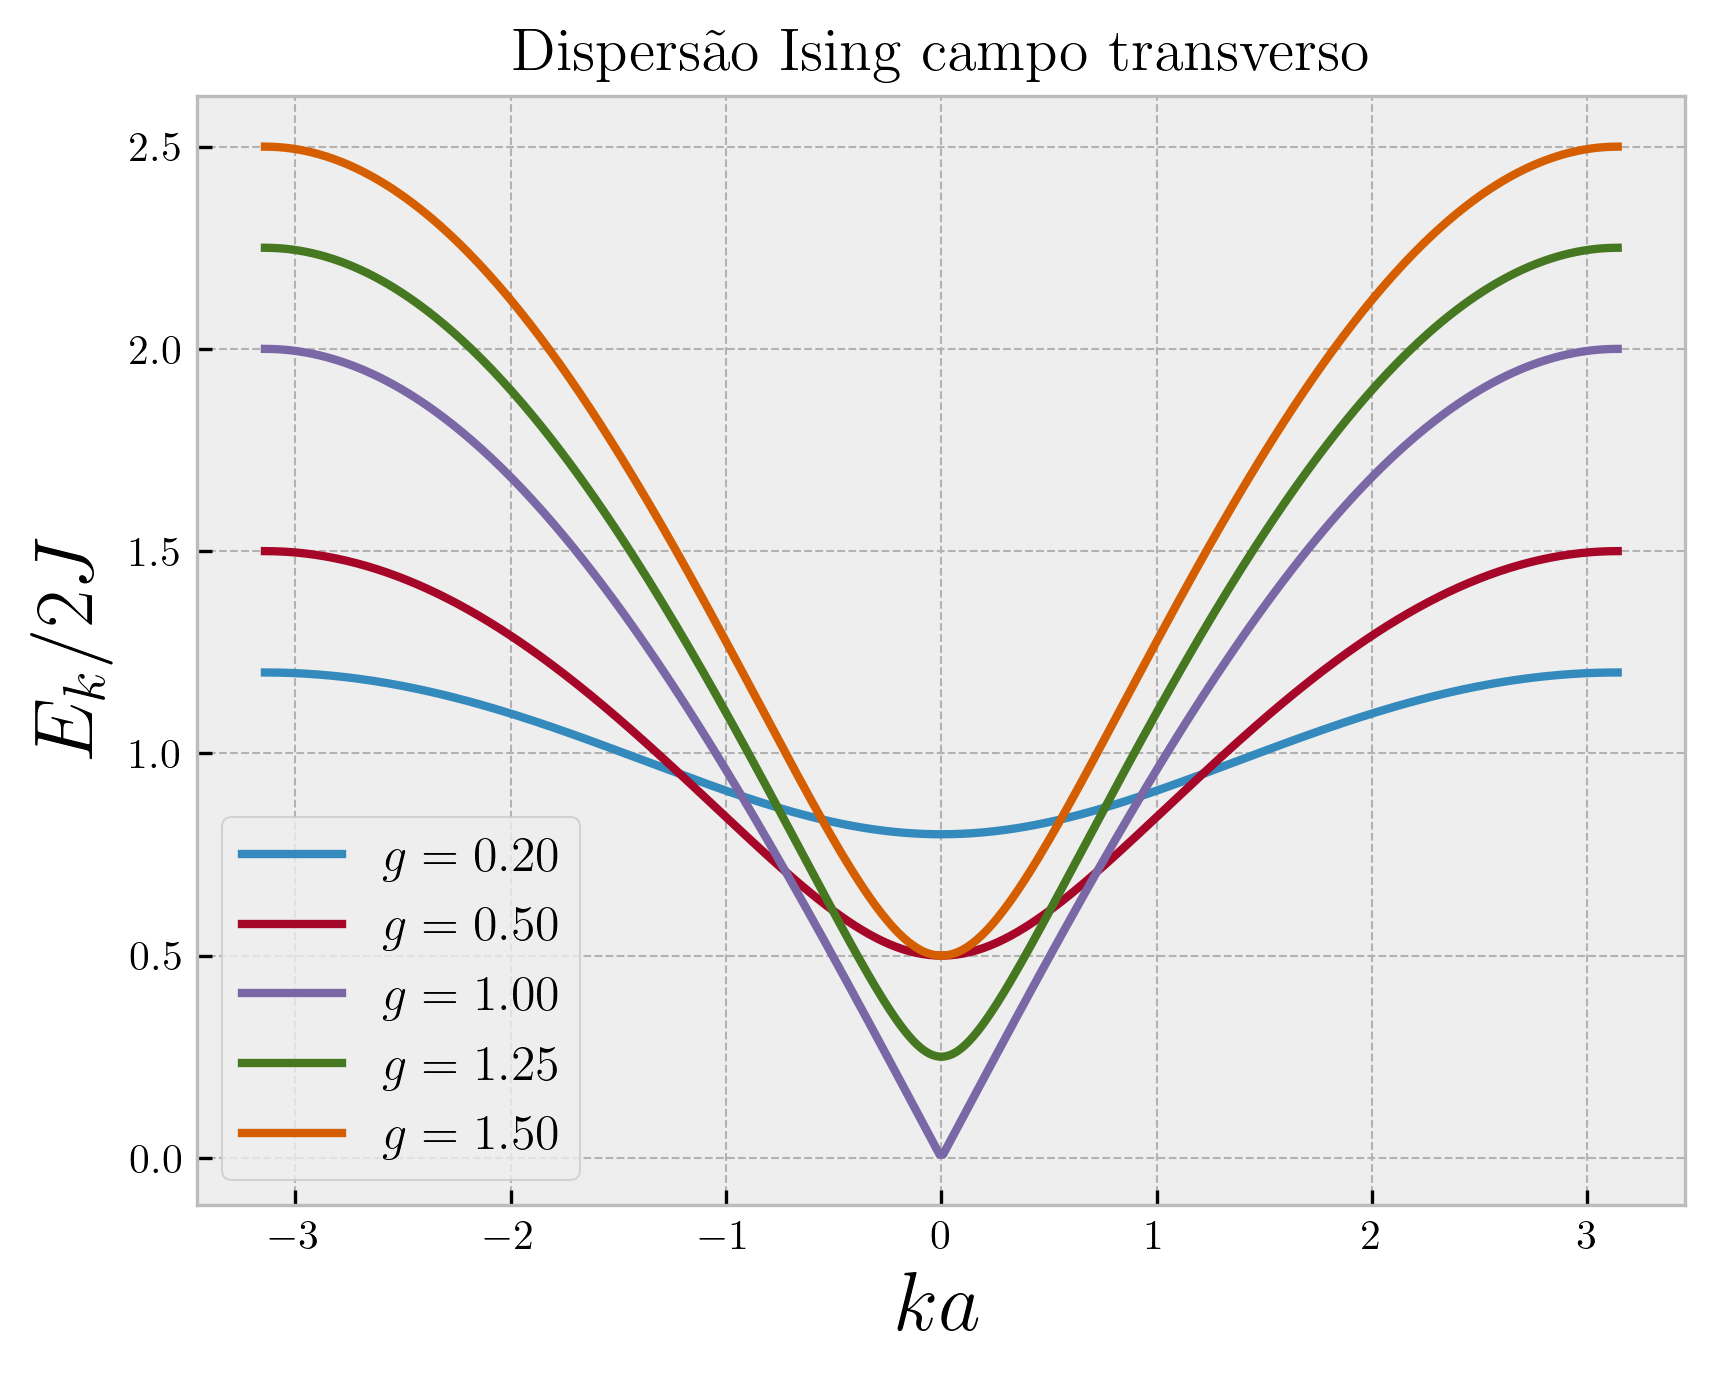
\includegraphics[width=0.6\linewidth]{fig/transv_ising2.png}
\caption{Dispersão $E_k$ para diferentes valores de $g$. No ponto $g_c = 1$ temos a transição de fase quântica, pois o gap fecha (a curva $E_k$ toca o zero).}
\label{fig:transv_ising2}
\end{figure}


Em nossas vimos que o comprimento de correlação é definido a partir do propagador $G(\k)$ que obtivemos considerando flutuações espaciais na teoria de Landau:
$$
G(\k) = \frac{k_B T / Ja^2}{k^2 + \xi^{-2}}.
$$

Veja que esse propagador é análogo a de uma partícula relativística, onde $G \propto \frac{1}{k^2 + m^2}$, de maneira que $\xi^{-1}$ faz o papel da massa $m$ da partícula. Por outro lado, se expandirmos $\cos(ka) \approx 1 - \frac{(ka)^2}{2}$ na dispersão $E_k$, nós obtemos
\begin{equation} \label{eq:approx-Ek}
E_k \approx 2J \sqrt{1 + g^2 - 2g \qty[1-\frac{(ka)^2}{2}]} =
\sqrt{g(2J a)^2 \, k^2 + [2J(g-1)]^2} = \sqrt{g(2J a)^2 \, k^2 + \Delta^2}.
\end{equation}
Veja que a dispersão aproximada acima tem a mesma forma de uma expressão relativística $\sqrt{k^2 + m^2}$ para uma partícula de massa $m$, onde a massa é proporcional ao gap $\Delta$.

\n

Percebendo então ambos $\xi^{-1}$ e $\Delta$ devem ser proporcionais à massa da quase-partícula $\gamma_k$, é razoável e correto tomar que $\xi^{-1} \propto \Delta \propto \abs{g-1} \implies \nu = 1$.

\n

Como observado no enunciado da prova, a energia do estado fundamental é
$$
E_0 = \ev{H}{0} = -\frac{1}{2} \sum_{k} E_k =
- \frac{N}{2a} \int_{-\pi}^{\pi} \frac{\dd{k}}{2\pi} 2J \sqrt{1 + g^2 - 2g\cos(ka)} =
- \frac{J N}{2a \pi} \int_{-\pi}^{\pi} \dd{k} \lambda_k.
$$

Usando a equação \ref{eq:approx-Ek} para $k\to 0$ e expandindo $\lambda_{k}(g) = \sqrt{1 + g^2 - 2g\cos(ka)} \approx \sqrt{ga^2 \, k^2 + (g-1)^2}$ ao redor de $g \approx g_c = 1$, temos
$$
\lambda_k(g) = \lambda_k(1) + \eval{\pdv{\lambda_k}{g}}_{g=1} (g-1) + \eval{\pdv[2]{\lambda_k}{g}}_{g=1} (g-1)^2 + O[(g-1)^3]
$$
$$
\lambda_k(g) = a\abs{k} + \frac{a}{2} \abs{k} (g-1) + \frac{a\abs{k}}{2} \qty(\frac{1}{(ka)^2} - \frac{1}{4}) (g-1)^2 + O[(g-1)^3]
$$
$$
\lambda_k(g) = \underbrace{a\abs{k}}_{\text{integrável}} \qty[1 + \frac{1}{2} (g-1) - \frac{1}{8} (g-1)^2 ] +
\frac{1}{2} (g-1)^2 \underbrace{\frac{1}{a\abs{k}}}_{\text{div. log.}} + \; O[(g-1)^3].
$$
Como $\ln x = \int \frac{\dd{x}}{x}$, vemos que o termo surgido $\displaystyle{\frac{1}{a\abs{k}}}$ faz com que $E_0$ tenha uma singularidade logaritmicamente em $k \to 0$.

\n

\section*{2) Mapa clássico quântico}

<++>



%%%-----
%%% Referências bibliográficas
%%%-----
%\addcontentsline{toc}{chapter}{\bibname}
%%\bibliographystyle{abntex2-num}
%\bibliography{citations}
%\bibliographystyle{ieeetr}


\end{document}
